% $Header: /home/vedranm/bitbucket/beamer/solutions/generic-talks/generic-ornate-15min-45min.en.tex,v 90e850259b8b 2007/01/28 20:48:30 tantau $

\documentclass{beamer}
  
% This file is a solution template for:

% - Giving a talk on some subject.
% - The talk is between 15min and 45min long.
% - Style is ornate.



% Copyright 2004 by Till Tantau <tantau@users.sourceforge.net>.
%
% In principle, this file can be redistributed and/or modified under
% the terms of the GNU Public License, version 2.
%
% However, this file is supposed to be a template to be modified
% for your own needs. For this reason, if you use this file as a
% template and not specifically distribute it as part of a another
% package/program, I grant the extra permission to freely copy and
% modify this file as you see fit and even to delete this copyright
% notice. 


\mode<presentation>
{
  \usetheme{Hannover}
  \usecolortheme{crane}

  \setbeamercovered{transparent}
  % or whatever (possibly just delete it)
}
\usepackage{amsmath}

\usepackage[english]{babel}
% or whatever

\usepackage[latin1]{inputenc}
% or whatever

\usepackage{times}
\usepackage[T1]{fontenc}
% Or whatever. Note that the encoding and the font should match. If T1
% does not look nice, try deleting the line with the fontenc.


\title[Governing Equations] % (optional, use only with long paper titles)
{The Physics of Simple Waves}

\subtitle
{Shock Waves} % (optional)

\author[Manuel Diaz] % (optional, use only with lots of authors)
{Manuel Diaz\inst{1} }
% - Use the \inst{?} command only if the authors have different
%   affiliation.

\institute[National Taiwan University] % (optional, but mostly needed)
{
  \inst{1}%
  National Taiwan University\\
  Institute of Applied Mechanics}
%  \and
%  \inst{2}%
%  Department of Theoretical Philosophy\\
%  University of Elsewhere}
% - Use the \inst command only if there are several affiliations.
% - Keep it simple, no one is interested in your street address.

\date[September 29th, 2011] % (optional)
{September 29th, 2011 / Weekly Meeting}

\subject{Talks}
% This is only inserted into the PDF information catalog. Can be left
% out. 



% If you have a file called "university-logo-filename.xxx", where xxx
% is a graphic format that can be processed by latex or pdflatex,
% resp., then you can add a logo as follows:

% \pgfdeclareimage[height=0.5cm]{university-logo}{university-logo-filename}
% \logo{\pgfuseimage{university-logo}}



% Delete this, if you do not want the table of contents to pop up at
% the beginning of each subsection:
%-------------------------------------------------------------------
%\AtBeginSubsection[]
%{
%  \begin{frame}<beamer>{Outline}
%    \tableofcontents[currentsection,currentsubsection]
%  \end{frame}
%}
%--------------------------------------------------------------------

% If you wish to uncover everything in a step-wise fashion, uncomment
% the following command: 

%\beamerdefaultoverlayspecification{<+->}


\begin{document}

\begin{frame}
  \titlepage
\end{frame}

\begin{frame}{Outline}
  \tableofcontents
  % You might wish to add the option [pausesections]
\end{frame}


% Since this a solution template for a generic talk, very little can
% be said about how it should be structured. However, the talk length
% of between 15min and 45min and the theme suggest that you stick to
% the following rules:  

% - Exactly two or three sections (other than the summary).
% - At *most* three subsections per section.
% - Talk about 30s to 2min per frame. So there should be between about
%   15 and 30 frames, all told.

\section{Introduction}

\subsection{Simple Waves}

\begin{frame}{WAVEFORM EXAMPLE 1}
  \begin{figure}
   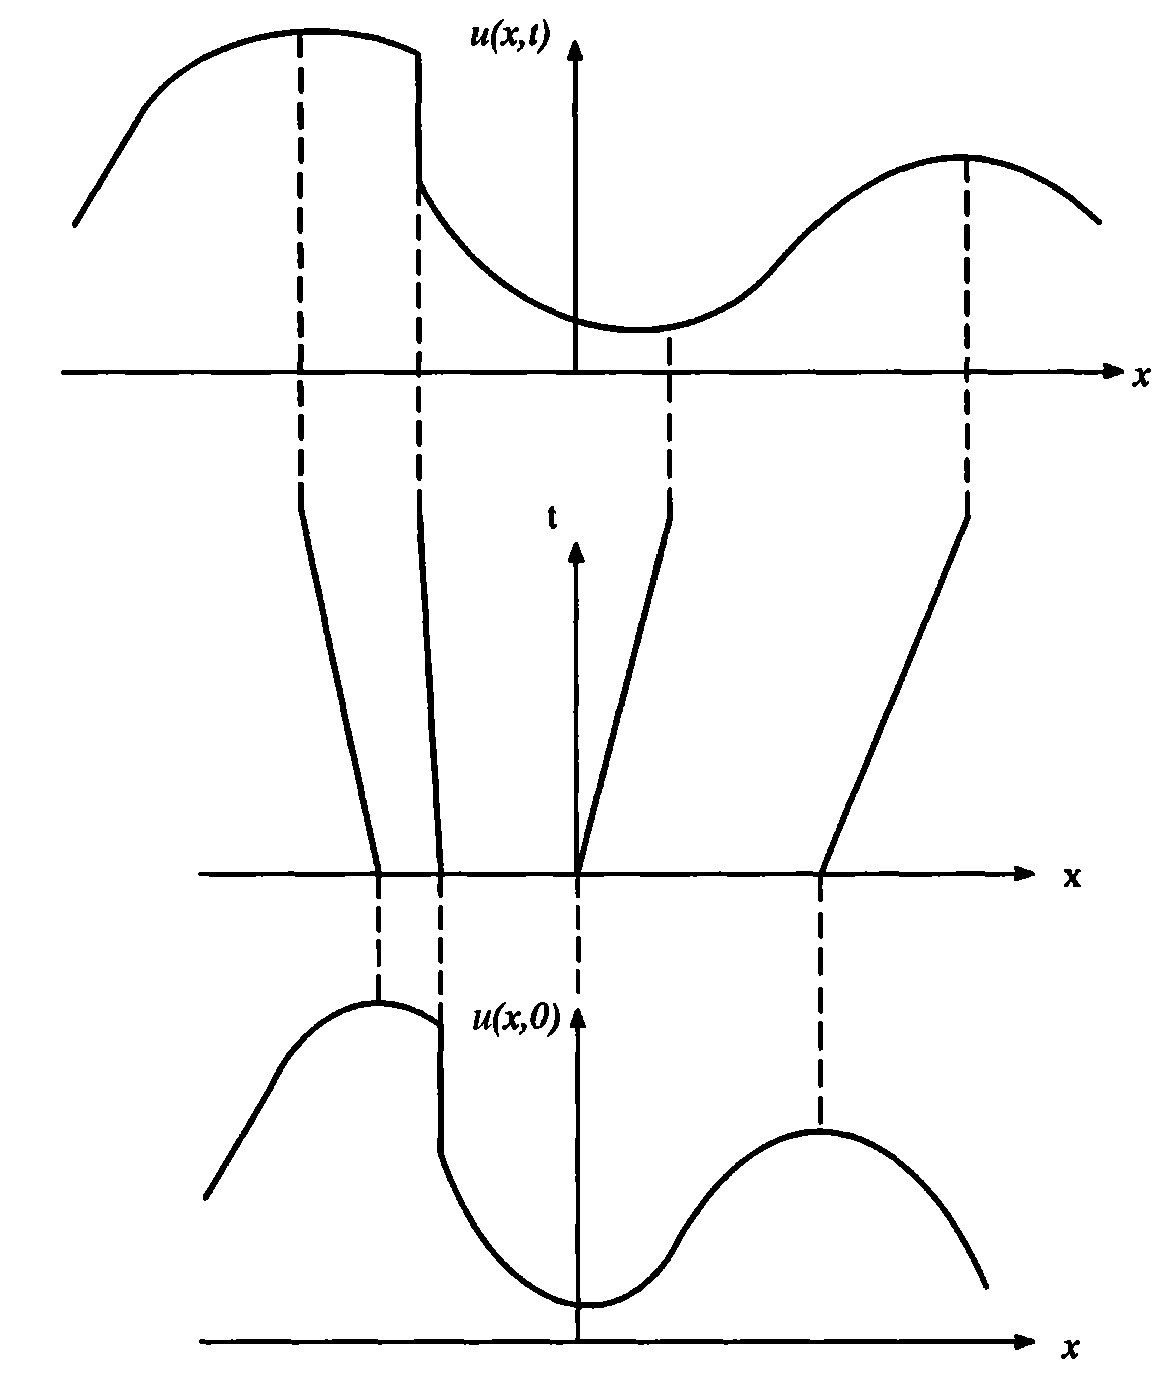
\includegraphics[scale=0.20]{figures/Preservation.jpg}
  \end{figure}
\end{frame}

\begin{frame}{WAVEFORM EXAMPLE 2}
  \begin{figure}
   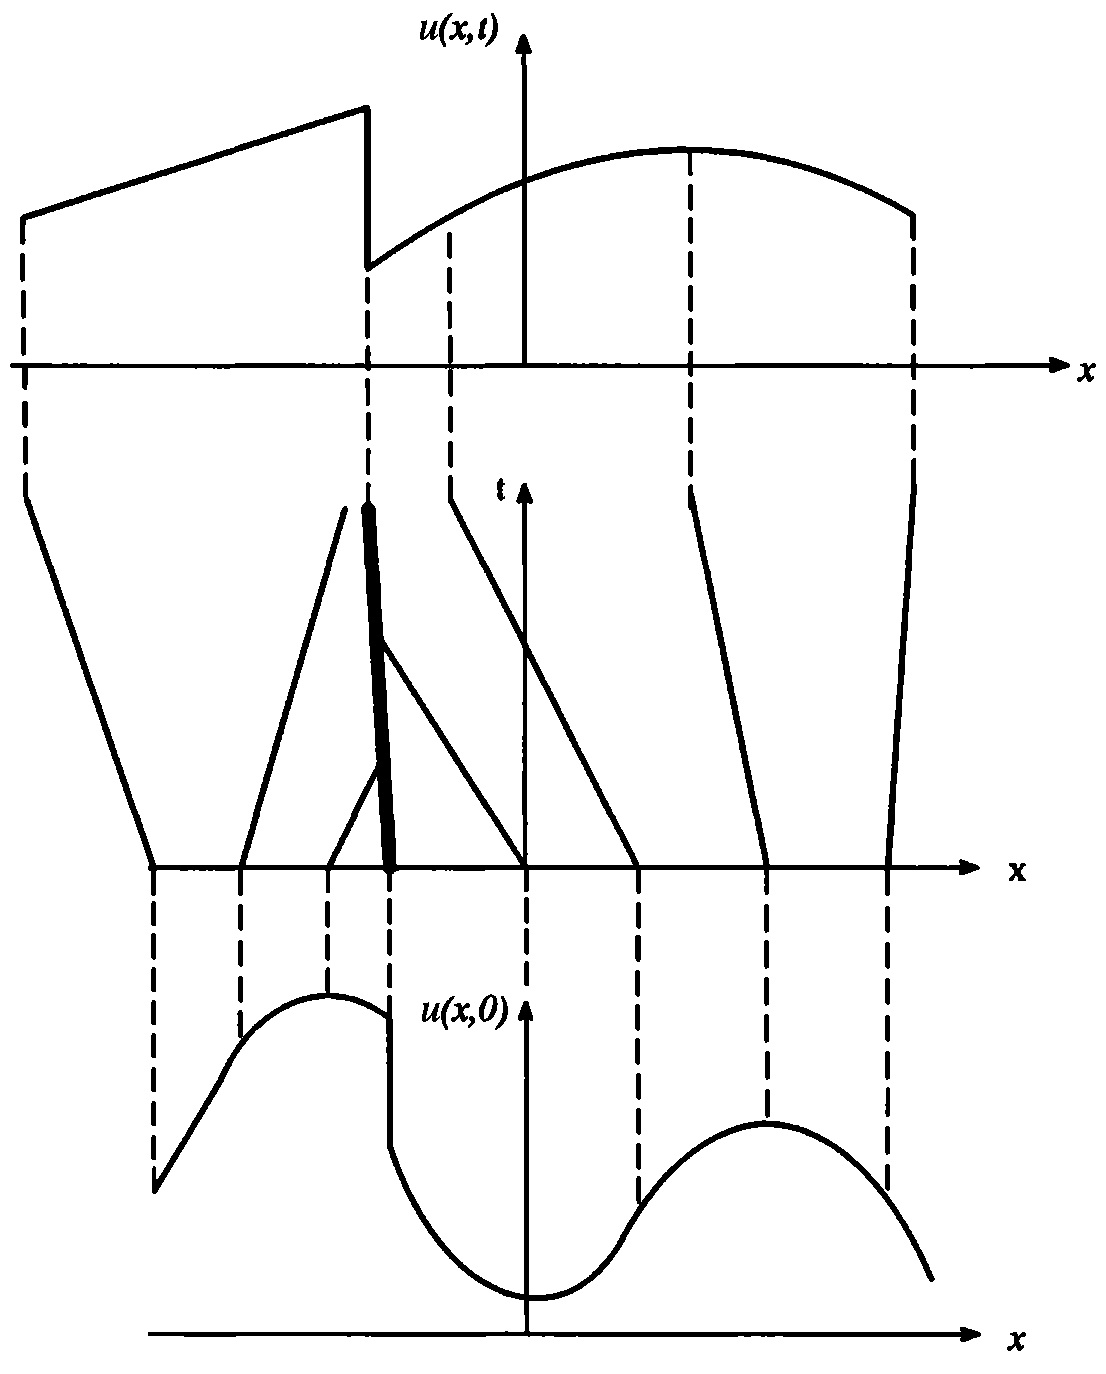
\includegraphics[scale=0.20]{figures/Destruction.jpg}
  \end{figure}
\end{frame}

\begin{frame}{WAVEFORM EXAMPLE 3}
  \begin{figure}
   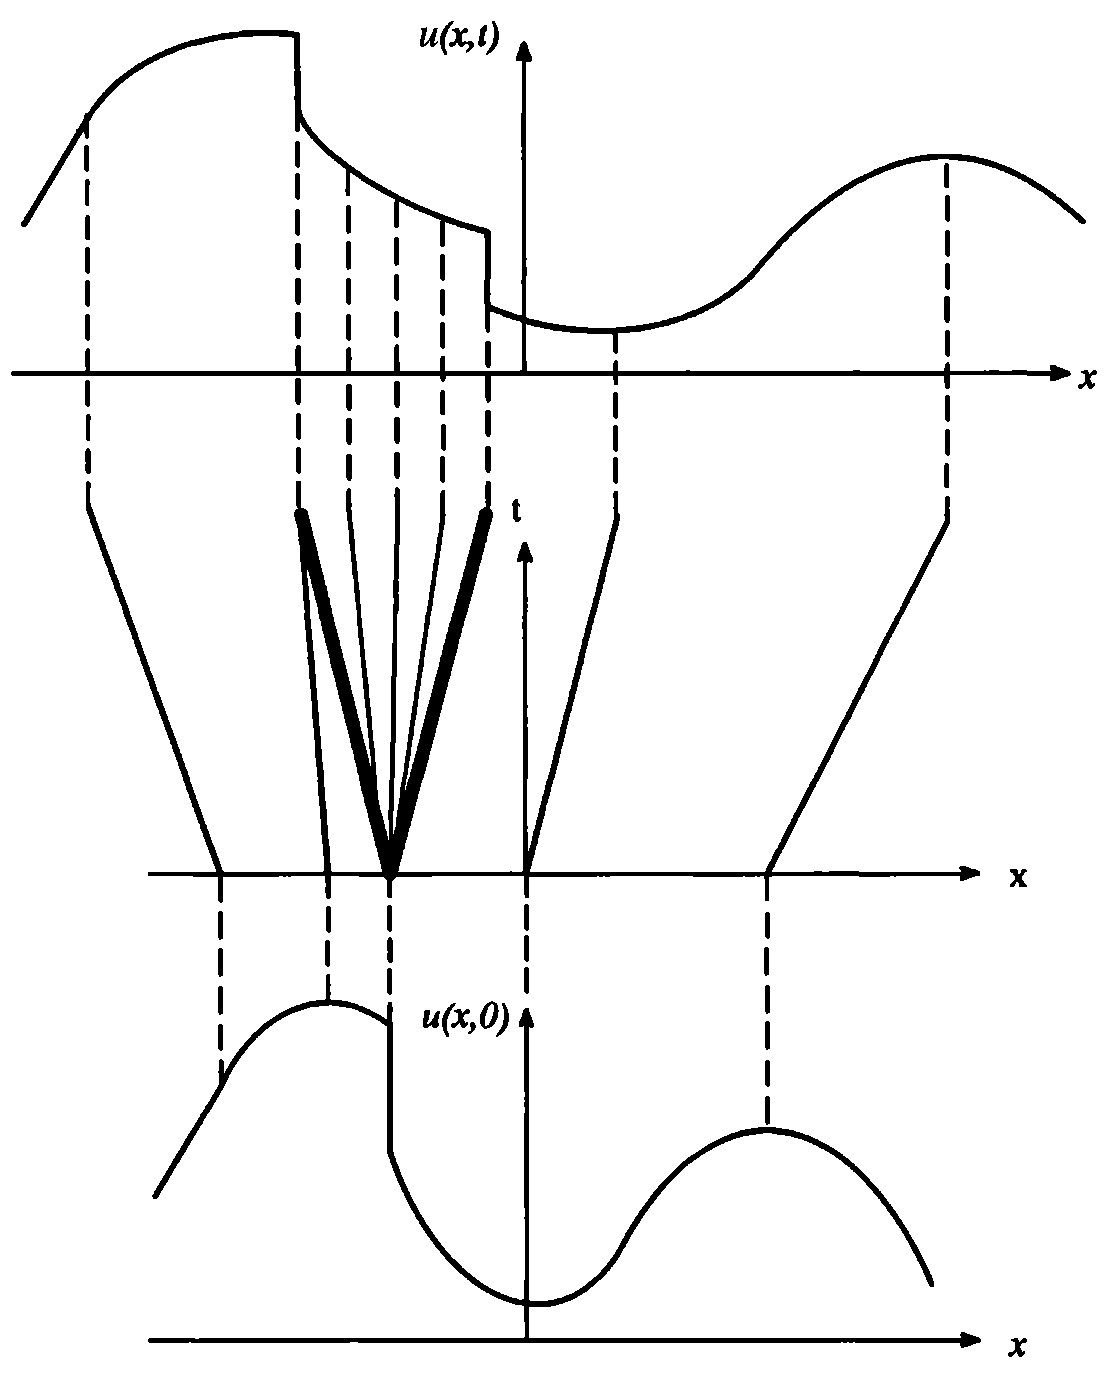
\includegraphics[scale=0.20]{figures/Creation.jpg}
  \end{figure}
\end{frame}

\begin{frame}{INTRODUCTION}
  \begin{itemize}
   \item Introduction to Simple Waves
  \end{itemize}
  \begin{figure}
   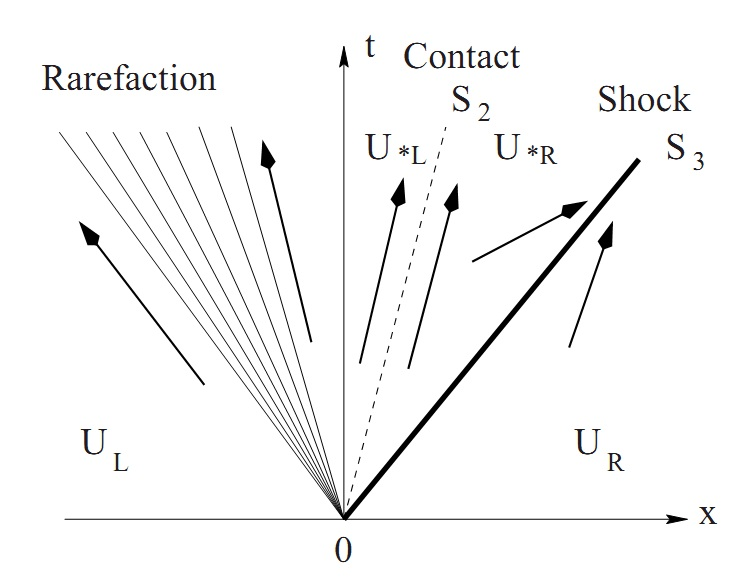
\includegraphics[scale=0.35]{figures/Simplewaves2.jpg}
  \end{figure}
\end{frame}

\section{Important Relations}

\subsection{Rankine-Hugoniot Relations}

\begin{frame}{RANKINE HUGONIOT RELATIONS}
  \begin{itemize}
   \item Rankine Hugoniot Relation help us to describe the behavior of shockwaves traveling normal to the prevaling flow.
  \end{itemize}
  \begin{equation}
   \vec{f}_R-\vec{f}_L=S(\vec{u}_R-\vec{u}_L)
  \end{equation}
\end{frame}

\begin{frame}{RANKINE HUGONIOT RELATIONS}{Vectors of conserved quantities}
  \begin{itemize}
   \item Vectors of conserved quantities:
  \end{itemize}
  \begin{equation}
    \vec{u} = \begin{bmatrix}
      {\rho} \\
      {\rho}{u} \\
      {\rho}{e_T}
    \end{bmatrix}=\begin{bmatrix}
      u_1\\ 
      u_2\\ 
      u_3
      \end{bmatrix}
  \end{equation}
  \begin{equation}
   \vec{f} = \begin{bmatrix}
      {\rho}{u} \\
      {\rho}{u^2}+p \\
      ({\rho}{e_T}+p)u
    \end{bmatrix}=\begin{bmatrix}
      f_1\\ 
      f_2\\ 
      f_3
      \end{bmatrix}
  \end{equation}
\end{frame}

\begin{frame}{RANKINE HUGONIOT RELATIONS}{Describing Shock Waves}
  \begin{itemize}
   \item Graphically:
  \end{itemize}
  \begin{figure}
   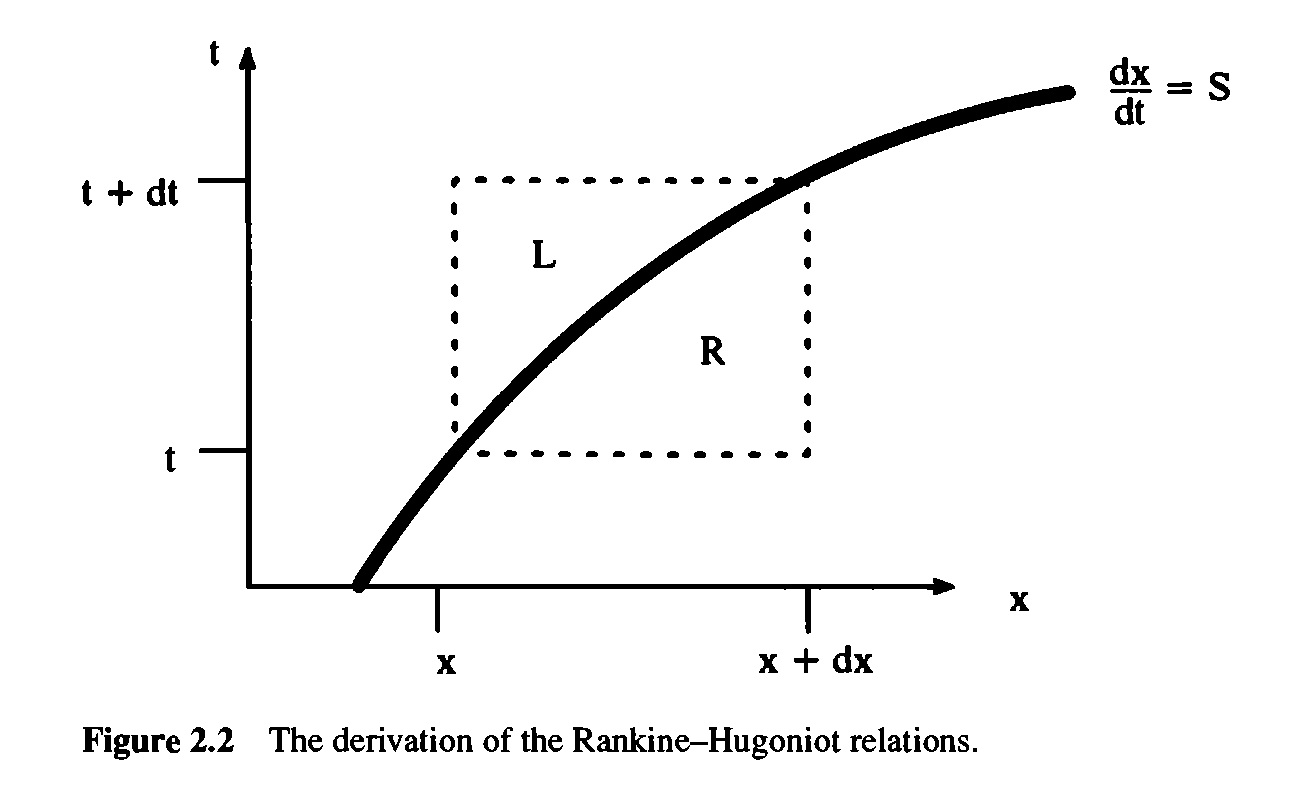
\includegraphics[scale=0.3]{figures/Rankine-Hugoniot.jpg}
  \end{figure}
\end{frame}

\begin{frame}{RANKINE HUGONIOT RELATIONS}{Describing Shock Waves}
  \begin{itemize}
   \item Suppose that a shock that separates two regions of uniform flow $u_l$ and $u_R$ is traveling at a constant speed.
  \end{itemize}
  \begin{eqnarray}
    &&\rho_L(u_L-S)=\rho_R(u_R-S) \\
    &&\rho_L(u_L-S)^2+p_L=\rho_R(u_R-S)^2+p_R \\
    &&\rho_L(u_L-S)(E_L)=\rho_R(u_R-S)(E_R) \nonumber
  \end{eqnarray}
\end{frame}

\begin{frame}{RANKINE HUGONIOT RELATIONS}{Describing Shock Waves}
  \begin{itemize}
   \item we notice that the energy relation can be simplified by using relation \alert{(4)} and:
  \end{itemize}
  \begin{equation}
    E=\frac{1}{2}u^2+h \nonumber
  \end{equation}
  \begin{itemize}
   \item Which would lead us to a prefered form of the energy description:
  \end{itemize}
  \begin{eqnarray}
    &&E_L=E_R \nonumber \\
    && \nonumber \\
    &&\frac{1}{2}(u_L-S)^2+h_L=\frac{1}{2}(u_R-S)^2+h_R \nonumber
  \end{eqnarray}
\end{frame}

\begin{frame}{RANKINE HUGONIOT RELATIONS}{Describing Shock Waves}
  \begin{itemize}
   \item Suppose that a shock that separates two regions of uniform flow $u_l$ and $u_R$ is traveling at a constant speed S.
  \end{itemize}
  \begin{eqnarray}
    &&\rho_L(u_L-S)=\rho_R(u_R-S) \nonumber \\
    &&\rho_L(u_L-S)^2+p_L=\rho_R(u_R-S)^2+p_R \nonumber \\
    &&\frac{1}{2}(u_L-S)^2+h_L=\frac{1}{2}(u_R-S)^2+h_R 
  \end{eqnarray}
\end{frame}

\subsection{Shockwave Relations}

\begin{frame}{SHOCKWAVE RELATIONS}
  \begin{itemize}
   \item We are basically targeting three main relations to describe the physics of the shock wave:
      \begin{itemize}
	\item Energy Relation:  $\rho_R$ and $\rho_L$
	\item Flux Relation:  $u_R$ and $u_L$
	\item Pressure Relation:  $P_R$ and $P_L$
      \end{itemize}
    \vskip0pt plus.5fill
    \item To do so, we start with Equations that we derive from the Hugoniot Relation, to formulate a way to describe this relations.
  \end{itemize}  
\end{frame}

\begin{frame}{SHOCKWAVE RELATIONS}
  \begin{itemize}
   \item Combining the eqns \alert{(4)} \& \alert{(5)}
  \end{itemize}  
  \begin{equation}
   \rho_L\left(\frac{\rho_R}{\rho_L}(u_R-S)^2\right)=\rho_R(u_R-S)^2 +P_R-P_L \nonumber
  \end{equation}
  \begin{itemize}
   \item we can develop the following two relations:
  \end{itemize}
  \begin{eqnarray}
   &&(u_R-S)^2=\frac{\rho_L}{\rho_R}\left ( \frac{P_R-P_L}{\rho_R-\rho_L} \right ) \\
   &&(u_L-S)^2=\frac{\rho_R}{\rho_L}\left ( \frac{P_R-P_L}{\rho_R-\rho_L} \right )
  \end{eqnarray}
\end{frame}

\begin{frame}{SHOCKWAVE RELATIONS}
  \begin{itemize}
   \item Substituting \alert{(7)} and \alert{(8)} in \alert{(6)}:
  \end{itemize}  
  \begin{equation}
   \frac{1}{2}(u_L-S)^2+h_L=\frac{1}{2}(u_R-S)^2+h_R \nonumber
  \end{equation}
  \begin{itemize}
   \item we can get now get a relation of enthalpies:
  \end{itemize}
  \begin{equation}
   \frac{1}{2}\left(P_L-P_R\right)\left(\frac{1}{\rho_L}+\frac{1}{\rho_R}\right)=h_R-h_L
  \end{equation}
\end{frame}

\begin{frame}{SHOCKWAVE RELATIONS}
  \begin{itemize}
   \item Now using the general formulation of enthalpies:
  \end{itemize}  
  \begin{equation}
   h=e+\frac{P}{\rho} \nonumber
  \end{equation}
  \begin{itemize}
   \item where $e$ is internal energy,
   \vskip0pt plus.5fill
   \item By performing some algebraic manipulations we can obtain:
  \end{itemize}
  \begin{equation}
   \frac{1}{2}\left(P_L+P_R\right)\left(\frac{1}{\rho_L}-\frac{1}{\rho_R}\right)=e_R-e_L 
  \end{equation}
  \begin{itemize}
   \item we have obtain the first of the relations we need.
  \end{itemize}
\end{frame}

\begin{frame}{SHOCKWAVE RELATIONS}
  \begin{itemize}
   \item but we know that: 
  \end{itemize}
  \begin{equation}
   \begin{matrix}
    e=c_vT, & c_v=\frac{R}{\gamma-1}, & P=\rho RT 
   \end{matrix}\nonumber
  \end{equation}
  \begin{itemize}
   \item Therefore we can describe internal energy as:
  \end{itemize}
  \begin{equation}
    e=\frac{P}{(\gamma-1)\rho} \nonumber
  \end{equation}
\end{frame}

\begin{frame}{SHOCKWAVE RELATIONS}
  \begin{itemize}
   \item Substituting the new formulation of internal energy in \alert{(10)}
  \end{itemize}  
  \begin{equation}
   \frac{1}{2}\left(P_L+P_R\right)\left(\frac{1}{\rho_L}-\frac{1}{\rho_R}\right)=e_R-e_L \nonumber
  \end{equation}
  \begin{itemize}
   \item and performing some algebraic manipulations we can obtain:
  \end{itemize}
  \begin{equation}
   \frac{\rho_L}{\rho_R}=\frac{\left(\frac{P_L}{P_R}\right)+\left(\frac{\gamma-1}{\gamma+1}\right)}{\left(\frac{\gamma-1}{\gamma+1}\right)\left(\frac{P_L}{P_R}\right)+1}
  \end{equation}
  \begin{itemize}
   \item Wich stablish a very useful relation between the density ratio $\rho_L/ \rho_R$
  \end{itemize}
\end{frame}

\begin{frame}{SHOCKWAVE RELATIONS}
  \begin{itemize}
   \item We wish to derivate a relation $P_L$ \& $P_R$; but first, it is convenient to develope a relation $a_L/a_R$ using the $\rho_L/ \rho_R$ ratio that we already now.
   \item using the general fomulation of sound speed "a" for a perfect gas:
  \end{itemize}  
  \begin{eqnarray}
    a=\gamma RT=\frac{\gamma P}{\rho} \nonumber \\
    \frac{a_R^2}{a_L^2}=\frac{P_R}{P_L}\left ( \frac{\rho_L}{\rho_R} \right ) \nonumber
  \end{eqnarray}
\end{frame}

\begin{frame}{SHOCKWAVE RELATIONS}
  \begin{itemize}
   \item and performing some algebraic manipulations we can obtain:
  \end{itemize}
  \begin{equation}
    \frac{a_R^2}{a_L^2}=\frac{P_R}{P_L}\left (\frac{\left(\frac{P_L}{P_R}\right)+\left(\frac{\gamma-1}{\gamma+1}\right)}{\left(\frac{\gamma-1}{\gamma+1}\right)\left(\frac{P_L}{P_R}\right)+1}  \right )
  \end{equation}
  \begin{itemize}
   \item We now introduce Mach Numbers
  \end{itemize}
  \begin{equation}
   \begin{matrix}
    M_R=u_R/a_R & M_{shock}=S/a_R
   \end{matrix} \nonumber
  \end{equation}
  \begin{itemize}
   \item Which would leads to:
  \end{itemize}
  \begin{equation}
   M_R-M_{shock}=\frac{u_R-S}{a_R}
  \end{equation}
\end{frame}

\begin{frame}{SHOCKWAVE RELATIONS}
  \begin{itemize}
   \item By manipulating eqns: \alert{(7)}, \alert{(11)} and \alert{(13)}:
  \end{itemize}
  \begin{eqnarray}
    && (u_R-S)^2=\frac{\rho_L}{\rho_R}\left ( \frac{P_R-P_L}{\rho_R-\rho_L} \right )\nonumber \\
    && \nonumber\\
    && \frac{\rho_L}{\rho_R}=\frac{\left(\frac{P_L}{P_R}\right)+\left(\frac{\gamma-1}{\gamma+1}\right)}{\left(\frac{\gamma-1}{\gamma+1}\right)\left(\frac{P_L}{P_R}\right)+1}\nonumber \\
    && \nonumber\\
    && M_R-M_{shock}=\frac{u_R-S}{a_R} \nonumber
  \end{eqnarray}
\end{frame}

\begin{frame}{SHOCKWAVE RELATIONS}
  \begin{itemize}
   \item theory leads us to the density and pressure ratios across the shock as functions of the relative Mach Number $M_R-M_{Shock}$, namely
  \end{itemize}
  \begin{eqnarray}
    &&\frac{\rho_L}{\rho_R}=\frac{(\gamma+1)(M_R-M_{shock})^2}{(\gamma-1)(M_R-M_{shock})^2+2}\\
    &&\nonumber \\
    &&\frac{P_L}{P_R}=\frac{2\gamma(M_R-M_{shock})^2-(\gamma-1)}{\gamma+1}
  \end{eqnarray}
\end{frame}

\begin{frame}{SHOCKWAVE RELATIONS}
  \begin{itemize}
   \item from \alert{(15)} we can notice the following relation:
  \end{itemize}
  \begin{equation}
   M_R-M_{shock}=-\sqrt{\left ( \frac{\gamma+1}{2\gamma} \right )\left ( \frac{P_L}{P_R} \right )+\left ( \frac{\gamma-1}{2\gamma} \right )}
  \end{equation}
  \begin{itemize}
   \item which leads to an expresion for the shock speed as a function of the pressure ratio across the shock, namely
  \end{itemize}
  \begin{equation}
   S=u_R+a_R\sqrt{\left ( \frac{\gamma+1}{2\gamma} \right )\left ( \frac{P_L}{P_R} \right )+\left ( \frac{\gamma-1}{2\gamma} \right )}
  \end{equation}
  \begin{itemize}
   \item Is important to notice that at $P_L/P_R$ aproaches unity it aproaches the characteristic speed $\lambda_+=u_R+a_R$ as expected.
  \end{itemize}
\end{frame}

\begin{frame}{SHOCKWAVE RELATIONS}
  \begin{itemize}
   \item we can relate the $u_L$ and $u_R$ by using \alert{(4)}
  \end{itemize}
  \begin{equation}
   \rho_L(u_L-S)=\rho_R(u_R-S)
  \end{equation}
  \begin{itemize}
   \item which leads to an expresion for $u_L$, namely
  \end{itemize}
  \begin{equation}
   u_L=\left (1-\frac{\rho_R}{\rho_L}  \right )S+u_R\left ( \frac{\rho_R}{\rho_L} \right )
  \end{equation}
  \begin{itemize}
   \item which leads to today's last relation:
  \end{itemize}
  \begin{equation}
   u_L=u_R+\frac{a_R}{\gamma}\frac{\frac{P_L}{P_R}-1}{\sqrt{\left ( \frac{\gamma+1}{2\gamma} \right )\left ( \frac{P_L}{P_R} \right )+\left ( \frac{\gamma-1}{2\gamma} \right )}}
  \end{equation}
\end{frame}

\subsection{Remarks}

\begin{frame}{Remarks}
  \begin{itemize}
   \item Shockwaves to the left or to the right?
  \end{itemize}
  \begin{figure}
   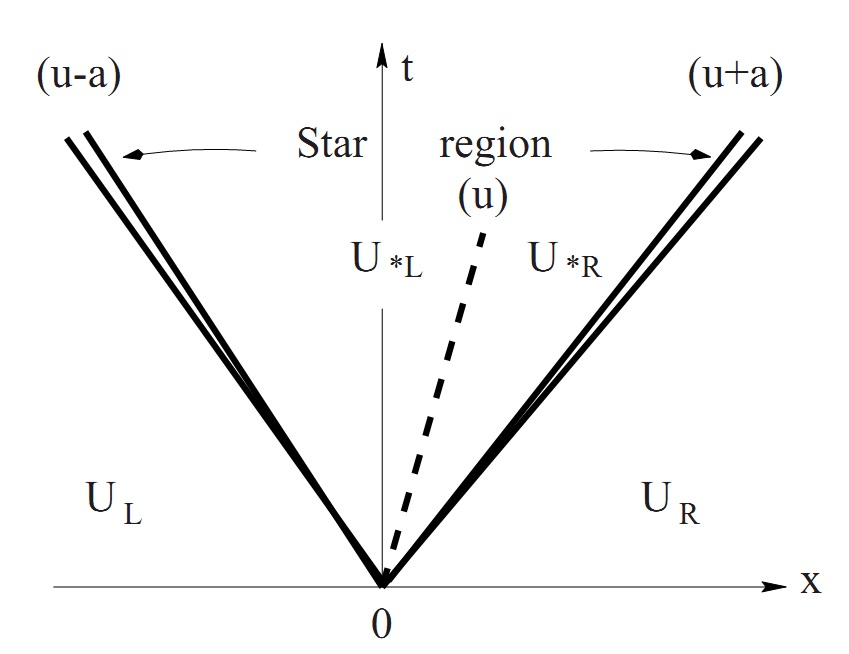
\includegraphics[scale=0.35]{figures/Simplewaves.jpg}
  \end{figure}
\end{frame}

\begin{frame}{Remarks}

   % Keep the summary *very short*.
  \begin{itemize}
  \item Some literature like to use the following notation for the Rigth running Shockwave:
  \end{itemize}
      \begin{eqnarray}
      && \frac{\rho_*}{\rho_R}=\frac{\left(\frac{P_*}{P_R}\right)+\left(\frac{\gamma-1}{\gamma+1}\right)}{\left(\frac{\gamma-1}{\gamma+1}\right)\left(\frac{P_*}{P_R}\right)+1} \nonumber \\
      && \frac{\rho_*}{\rho_R}=\frac{(\gamma+1)(M_R-M_{shock})^2}{(\gamma-1)(M_R-M_{shock})^2+2} \nonumber \\
      && \nonumber \\
      && \frac{P_*}{P_R}=\frac{2\gamma(M_R-M_{shock})^2-(\gamma-1)}{\gamma+1} \nonumber \\
      && u_*=u_R+\frac{a_R}{\gamma}\frac{\frac{P_*}{P_R}-1}{\sqrt{\left ( \frac{\gamma+1}{2\gamma} \right )\left ( \frac{P_*}{P_R} \right )+\left ( \frac{\gamma-1}{2\gamma} \right )}} \nonumber
    \end{eqnarray}
\end{frame}

\begin{frame}{Remarks}

   % Keep the summary *very short*.
  \begin{itemize}
  \item For the left running Shockwave, the equations are totally analogous:
  \end{itemize}
      \begin{eqnarray}
      && \frac{\rho_*}{\rho_L}=\frac{\left(\frac{P_*}{P_L}\right)+\left(\frac{\gamma-1}{\gamma+1}\right)}{\left(\frac{\gamma-1}{\gamma+1}\right)\left(\frac{P_*}{P_L}\right)+1} \nonumber \\
      && \frac{\rho_*}{\rho_L}=\frac{(\gamma+1)(M_R-M_{shock})^2}{(\gamma-1)(M_R-M_{shock})^2+2} \nonumber \\
      && \nonumber \\
      && \frac{P_*}{P_L}=\frac{2\gamma(M_L-M_{shock})^2-(\gamma-1)}{\gamma+1} \nonumber \\
      && u_*=u_L+\frac{a_L}{\gamma}\frac{\frac{P_*}{P_L}-1}{\sqrt{\left ( \frac{\gamma+1}{2\gamma} \right )\left ( \frac{P_*}{P_L} \right )+\left ( \frac{\gamma-1}{2\gamma} \right )}} \nonumber
    \end{eqnarray}
\end{frame}

\section*{Summary}

\begin{frame}{Summary}

   % Keep the summary *very short*.
  \begin{itemize}
  \item Equations \alert{(14)}, \alert{(15)} and \alert{(20)} define a shock for given initial conditions $(\rho_R,u_R,P_R)^T$ ahead of the shock and a chosen mach number $M_s$ or equivalently a shock Speed $S$.
  \end{itemize}
      \begin{eqnarray}
      && \frac{\rho_L}{\rho_R}=\frac{(\gamma+1)(M_R-M_{shock})^2}{(\gamma-1)(M_R-M_{shock})^2+2} \nonumber \\
      && \nonumber \\
      && \frac{P_L}{P_R}=\frac{2\gamma(M_R-M_{shock})^2-(\gamma-1)}{\gamma+1} \nonumber \\
      && u_L=u_R+\frac{a_R}{\gamma}\frac{\frac{P_L}{P_R}-1}{\sqrt{\left ( \frac{\gamma+1}{2\gamma} \right )\left ( \frac{P_L}{P_R} \right )+\left ( \frac{\gamma-1}{2\gamma} \right )}} \nonumber
    \end{eqnarray}
\end{frame}

\end{document}

\end{document}


